% CREATED BY DAVID FRISK, 2016
\documentclass[../../main.tex]{subfiles}
 
\begin{document}

% COVER PAGE
\begin{titlepage}
\newgeometry{top=3cm, bottom=3cm,
			left=2.25 cm, right=2.25cm}	% Temporarily change margins		
			
% Cover page background 
\AddToShipoutPicture*{\backgroundpic{-4}{56.7}{figure/auxiliary/frontpage_swe.pdf}}
\addtolength{\voffset}{2cm}

% Cover picture (replace with your own or delete)		
\begin{figure}[H]
\centering
\vspace{2cm}	% Adjust vertical spacing here
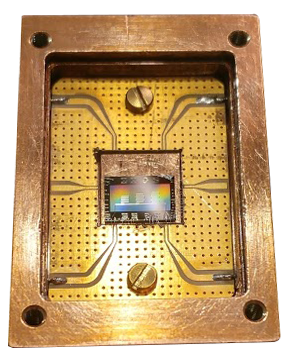
\includegraphics[width=0.5\linewidth]{figure/auxiliary/front_image.png}
\end{figure}

% Cover text
%\mbox{}
\renewcommand{\familydefault}{\sfdefault} \normalfont % Set cover page font
\textbf{{\Huge Lågpassfilter för supraledande \\mikrovågsresonatorer}}

{\Large \undertitel}

Kandidatarbete inom Teknisk fysik
\setlength{\parskip}{0.5cm}

{\Large PHILIP EDENBORG

\setlength{\parskip}{0em}
LINA HULTQUIST

MATTIAS SJÖSTEDT

JOHAN WINTHER

}

\setlength{\parskip}{1cm}

\department\\
\textsc{\university} \\
\adress

\renewcommand{\familydefault}{\rmdefault} \normalfont % Reset standard font
\end{titlepage}


% BACK OF COVER PAGE (BLANK PAGE)
\newpage\null\thispagestyle{empty}\newpage
\restoregeometry

%\mbox{}

% TITLE PAGE
\newpage
\thispagestyle{empty}
\begin{center}
	\textsc{\large \reportnr}\\[4cm]		% Report number given by department 
	\textbf{\Large \titel} \\[1cm]
	{\large \undertitel}\\[1cm]
	{\large PHILIP EDENBORG\\LINA HULTQUIST\\MATTIAS SJÖSTEDT\\JOHAN WINTHER}
	
	\vfill	
	% Logotype on titlepage	
	\begin{figure}[H]
	\centering
	% Remove the following line to remove the titlepage logotype
	
\includegraphics[width=0.2\pdfpagewidth]{figure/auxiliary/logo_swe.pdf} \\	
	\end{figure}	\vspace{5mm}	
	
    \department\\
	\emph{\division}\\
	%Name of research group (if applicable)\\
	\textsc{\university} \\
	\adress \\
\end{center}


% IMPRINT PAGE (BACK OF TITLE PAGE)
\newpage
\thispagestyle{plain}
\vspace*{4.5cm}
\titel\\
\undertitel\\
\newline
Philip Edenborg, Lina Hultquist, Mattias Sjöstedt, Johan Winther \setlength{\parskip}{1cm}
% Reduction of quasiparticle population

\copyright ~ Philip Edenborg, Lina Hultquist, Mattias Sjöstedt, Johan Winther, \the\year. \setlength{\parskip}{1cm}

\textbf{Handledare:}\\
Dr. Jonas Bylander, \department\\
Dr. Jonathan Burnett, \department\\
\textbf{Examinator:}\\
Dr. Vessen Vassilev, \department\setlength{\parskip}{1cm}

\reportnr\\	% Report number given by department 
\department\\
\division\\
%Name of research group (if applicable)\\
\university\\
SE-412 58 Göteborg\\
%Telephone +46 31 772 1000 \setlength{\parskip}{0.5cm}

\vfill
% Caption for cover page figure if used, possibly with reference to further information in the report
Framsida: Resonator på ett chip. Foto från Jonathan Burnett. \setlength{\parskip}{0.5cm}

Typsatt i \LaTeX \\
%Printed by [Name of printing company]\\
\adress

\end{document}